\documentclass[10pt,journal]{IEEEtran}
\usepackage{fontspec,xeCJK}
\setmainfont{Times New Roman}
\setsansfont{Arial}
\setmonofont{Consolas}
\setCJKmainfont{SimSun}[BoldFont=SimHei,ItalicFont=KaiTi,BoldItalicFont=SimHei]
\setCJKsansfont{SimHei}
\usepackage{amsmath,amssymb,graphicx,booktabs,array,tabularx,url,xurl,placeins,stfloats}
\urlstyle{same}
\usepackage[hidelinks]{hyperref}
\renewcommand{\abstractname}{摘要}
\renewcommand{\IEEEkeywordsname}{关键词}
\renewcommand{\tablename}{表}
\renewcommand{\figurename}{图}
\renewcommand{\refname}{参考记录}
\renewcommand{\arraystretch}{1.16}
\setlength{\tabcolsep}{3pt}
\setlength{\textfloatsep}{10pt plus 2pt minus 2pt}
\setlength{\dbltextfloatsep}{10pt plus 2pt minus 2pt}
\setlength{\floatsep}{8pt plus 2pt minus 1pt}
\renewcommand{\topfraction}{.92}
\renewcommand{\dbltopfraction}{.92}
\renewcommand{\textfraction}{.06}
\renewcommand{\floatpagefraction}{.8}
\renewcommand{\dblfloatpagefraction}{.8}
\setcounter{topnumber}{4}
\setcounter{dbltopnumber}{4}
\setcounter{totalnumber}{8}
\makeatletter
\setlength{\@fptop}{0pt}
\setlength{\@fpsep}{10pt}
\setlength{\@fpbot}{0pt plus 1fil}
\setlength{\@dblfptop}{0pt}
\setlength{\@dblfpsep}{10pt}
\setlength{\@dblfpbot}{0pt plus 1fil}
\makeatother
\clubpenalty=10000\widowpenalty=10000
\newcolumntype{Y}{>{\raggedright\arraybackslash}X}
\begin{document}
\title{PAMF与对比方法的重点实验分析}
\author{实验结果报告\quad 2026年10月26日}
\maketitle
\begin{abstract}
本报告按五类重点问题整理PAMF与四种完整对比方法的冻结结果。监督与普通PL主比较采用双柱，无增强仅报告CLEAN，有增强分列CLEAN和综合星地；其余主图固定增强半监督。所有适用图纳入单PAMF与PAMF+DURA，恢复网络泛用性也纳入PAMF。源数量以1至6折线表示，5源复用同种子主实验模型并汇总共同6个目标接收机。当前普通PL的无增强PAMF缺项明确标注；原补充图表保留在Excel。本次没有新增训练、预测或目标真值访问。
\end{abstract}
\begin{IEEEkeywords}
射频指纹识别，跨接收机泛化，普通伪标签，信道增强，信号恢复，分组评估。
\end{IEEEkeywords}
本版按用户指定的五类问题组织主结果：先配对比较监督与普通 PL 半监督，再报告启用星地增强的半监督泛化、七场景、1 至 6 个源接收机和 DURA 泛用性。PAMF 及 PAMF+DURA 以红、橙色突出；颜色不改变坐标、统计或缺项含义。其余既有图表完整保留在 Excel 的补充工作表。证据整理日期为 2026 年 10 月 26 日。

\section{实验定义与展示范围}
表~\ref{tab:grouped-1}~本版重点实验的固定条件。

\begin{table}[!htbp]
\caption{本版重点实验的固定条件}
\label{tab:grouped-1}
\centering
\footnotesize
\begin{tabularx}{\columnwidth}{YYY}
\toprule
\textbf{问题} & \textbf{训练条件} & \textbf{主图内容} \\
\midrule
监督与半监督 & 无增强、启用增强分别比较 & 无增强仅 CLEAN；有增强分别给 CLEAN 与综合星地 \\
接收机划分、标注比例、源数量 & 普通 PL 半监督＋星地增强 & 每个设置内 CLEAN／综合星地双柱；均含 PAMF 与 PAMF+DURA \\
七场景 & 普通 PL 半监督＋星地增强 & CLEAN、高/中/低郊区、高/中/低城市 \\
1 至 6 源折线 & 普通 PL 半监督＋星地增强 & 固定共同 6 目标；CLEAN 和综合星地分图 \\
DURA 泛用性 & 普通 PL 半监督＋星地增强 & 五种识别器各自未接入／接入恢复器双柱 \\
\bottomrule
\end{tabularx}
\end{table}
主比较方法为 RIEI、DRIFT、IB-RFF、SDG、PAMF、PAMF+DURA。前五项直接识别；PAMF+DURA 的实际顺序是先 DURA 恢复、再由同一 PAMF 识别器分类，不计为另一次识别器训练。外部方法接 DURA 的结果单列泛用性，不替换其主比较成绩。所有方法均保留原生完整目标、预算与默认分类头，不声称等计算比较。

普通 PL 采用当前模型 eval/no\_grad 硬标签，阈值 0.95、权重 1、整批无标签损失平均，无 EMA 教师或复杂筛选。PAMF 监督为 50 轮有标签训练，普通 PL 为 13 轮有标签＋37 轮联合训练，均为 11100 次更新。保留 PAMF 自身有标签目标与信道视图，不把监督版称为纯交叉熵。外部方法的三场景概率为 40\%/35\%/25\%，PAMF 主配方为三场景均匀；原生目标和增强剂量差异均保留。

综合星地指先在每个模型种子内平均六种 practical 的准确率，再计算三个模型种子的均值和样本标准差；CLEAN 不参加该平均。柱图和折线误差线均为模型种子样本标准差，不是置信区间或显著性结论。主图测试为目标接收机的已见日期跨接收机泛化；双跨、源接收机跨日诊断、Macro-F1、十类规模与时延等保留在 Excel 补充页。

数据来自 WiSig 地面代理。训练/源验证日期为 2021 年 3 月 8、15、23 日，3 月 1 日为更早的未见日期。仿真星地环境不是实测在轨链路。训练、选模和调度均不使用本次目标成绩反馈。

表~\ref{tab:grouped-2}~主要数据设置；监督组不读取无标签训练池。

\begin{table*}[!tbp]
\caption{主要数据设置；监督组不读取无标签训练池}
\label{tab:grouped-2}
\centering
\small
\begin{tabularx}{\textwidth}{YYYYYY}
\toprule
\textbf{设置} & \textbf{类数} & \textbf{源/原目标接收机数} & \textbf{有标签训练} & \textbf{无标签池} & \textbf{源验证} \\
\midrule
标准接收机划分 & 6 & 5/7 & 6300 & 56700 & 27000 \\
接收机划分一 & 6 & 5/7 & 6300 & 56700 & 27000 \\
接收机划分二 & 6 & 5/7 & 6300 & 56700 & 27000 \\
1\%标注 & 6 & 5/7 & 630 & 62370 & 27000 \\
5\%标注 & 6 & 5/7 & 3150 & 59850 & 27000 \\
1个源接收机 & 6 & 1/6 & 1260 & 11340 & 5400 \\
2个源接收机 & 6 & 2/6 & 2520 & 22680 & 10800 \\
3个源接收机 & 6 & 3/6 & 3780 & 34020 & 16200 \\
4个源接收机 & 6 & 4/6 & 5040 & 45360 & 21600 \\
6个源接收机 & 6 & 6/6 & 7560 & 68040 & 32400 \\
\bottomrule
\end{tabularx}
\end{table*}
\section{监督与普通 PL 的双柱比较}
无增强主图保留五种识别方法。此前导出没有纳入的 PAMF 无增强监督结果现已从完整冻结包补回，仍保留其原有监督参照配方；当前普通 PL 的匹配无增强结果不存在，按用户要求明确留缺，不填零、不用旧复杂半监督或已退出方法替代。PAMF 无增强监督参照与有增强主配方还存在辅助槽差异，因此两图之间的分差不能全部解释为信道增强的因果效果。

表~\ref{tab:grouped-3}~无增强、标准主划分、目标跨接收机 CLEAN 准确率（\%）。

\begin{table}[!htbp]
\caption{无增强、标准主划分、目标跨接收机 CLEAN 准确率（\%）}
\label{tab:grouped-3}
\centering
\footnotesize
\begin{tabularx}{\columnwidth}{YYY}
\toprule
\textbf{识别方法} & \textbf{监督} & \textbf{普通 PL 半监督} \\
\midrule
RIEI & 66.93\ensuremath{\pm}0.71 & 67.28\ensuremath{\pm}0.88 \\
DRIFT & 66.21\ensuremath{\pm}3.30 & 67.69\ensuremath{\pm}1.71 \\
IB-RFF & 66.29\ensuremath{\pm}1.40 & 66.44\ensuremath{\pm}2.90 \\
SDG & 74.25\ensuremath{\pm}0.88 & 74.64\ensuremath{\pm}0.14 \\
PAMF & 85.41\ensuremath{\pm}0.74 & 缺项 \\
\bottomrule
\end{tabularx}
\end{table}
\begin{figure*}[!tbp]
\centering
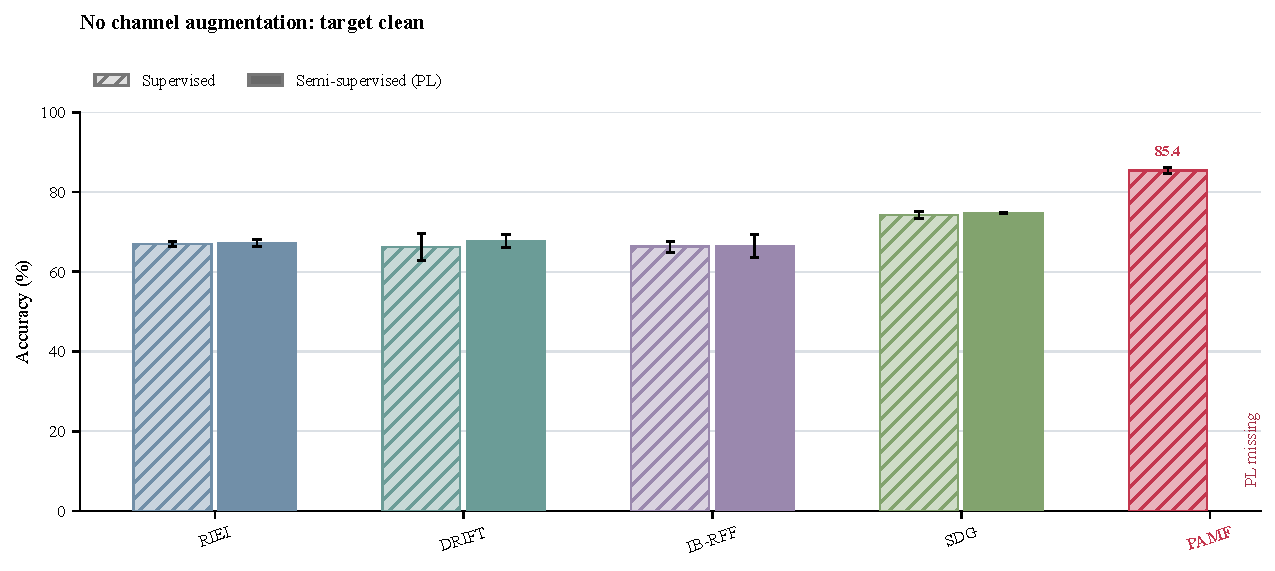
\includegraphics[width=\textwidth]{../figures/main_no_channel.pdf}
\caption{无附加星地增强的监督／普通 PL 双柱比较，仅报告目标 CLEAN。PAMF 监督柱为既有无增强参照，普通 PL 缺项以文字标出，未填零值。}
\label{fig:grouped-1}
\end{figure*}
表~\ref{tab:grouped-4}~启用星地增强的标准主划分准确率（\%）；两类测试各自配对。

\begin{table*}[!tbp]
\caption{启用星地增强的标准主划分准确率（\%）；两类测试各自配对}
\label{tab:grouped-4}
\centering
\small
\begin{tabularx}{\textwidth}{YYYYY}
\toprule
\textbf{方法} & \textbf{监督 CLEAN} & \textbf{PL CLEAN} & \textbf{监督综合星地} & \textbf{PL 综合星地} \\
\midrule
RIEI & 62.22\ensuremath{\pm}1.53 & 61.63\ensuremath{\pm}1.89 & 50.08\ensuremath{\pm}1.60 & 49.95\ensuremath{\pm}1.55 \\
DRIFT & 61.77\ensuremath{\pm}6.73 & 66.12\ensuremath{\pm}3.20 & 55.22\ensuremath{\pm}5.28 & 56.76\ensuremath{\pm}2.29 \\
IB-RFF & 66.74\ensuremath{\pm}2.61 & 66.63\ensuremath{\pm}2.29 & 53.10\ensuremath{\pm}1.83 & 52.57\ensuremath{\pm}2.17 \\
SDG & 73.18\ensuremath{\pm}2.16 & 74.32\ensuremath{\pm}1.52 & 65.16\ensuremath{\pm}2.03 & 65.30\ensuremath{\pm}1.14 \\
PAMF & 85.94\ensuremath{\pm}0.84 & 86.04\ensuremath{\pm}0.36 & 71.29\ensuremath{\pm}0.90 & 71.05\ensuremath{\pm}0.91 \\
PAMF+DURA & 85.93\ensuremath{\pm}0.85 & 86.08\ensuremath{\pm}0.34 & 77.36\ensuremath{\pm}0.55 & 78.52\ensuremath{\pm}0.12 \\
\bottomrule
\end{tabularx}
\end{table*}
\begin{figure*}[!tbp]
\centering
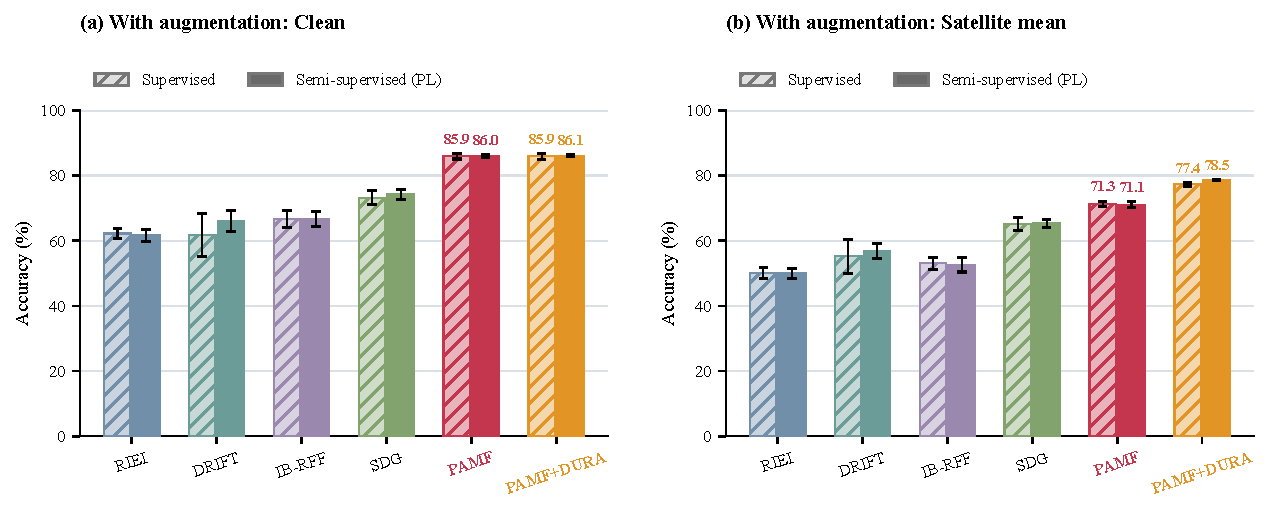
\includegraphics[width=\textwidth]{../figures/main_channel_on.pdf}
\caption{启用星地增强后，监督和普通 PL 半监督按方法配对；(a) CLEAN，(b) 六种 practical 的平均准确率。两幅均列单 PAMF 与 PAMF+DURA。监督恢复器只用有标签源 IQ，半监督恢复器可用全部允许源训练 IQ。}
\label{fig:grouped-2}
\end{figure*}
在固定的增强半监督主比较中，PAMF 的综合星地准确率为 71.05\ensuremath{\pm}0.91\%，高于四种直接识别外部方法中的最高均值 65.30\%；接入 DURA 后为 78.52\ensuremath{\pm}0.12\%。普通 PL 相对 PAMF 监督的直接识别均值变化为 -0.24 个百分点，故该结果不支持把 PAMF 的全部优势归因于普通 PL。两种学习组的恢复器源 IQ 权限也不同，不能将完整系统的跨组差全部归因于识别器伪标签。

\section{接收机划分、标注比例与源数量}
本节全部使用普通 PL 半监督＋训练星地增强。每个数据设置均列六个主比较项，以 CLEAN／综合星地双柱展示；PAMF 不再只出现在标准划分图。三个接收机划分都为 5 源/7 目标，三套源集合两两仅交一个接收机；每个模型和恢复器均匹配该划分。标注比例为源训练池的 1\%/5\%/10\%，对应 630/3150/6300 个有标签包。

\begin{figure*}[!tbp]
\centering
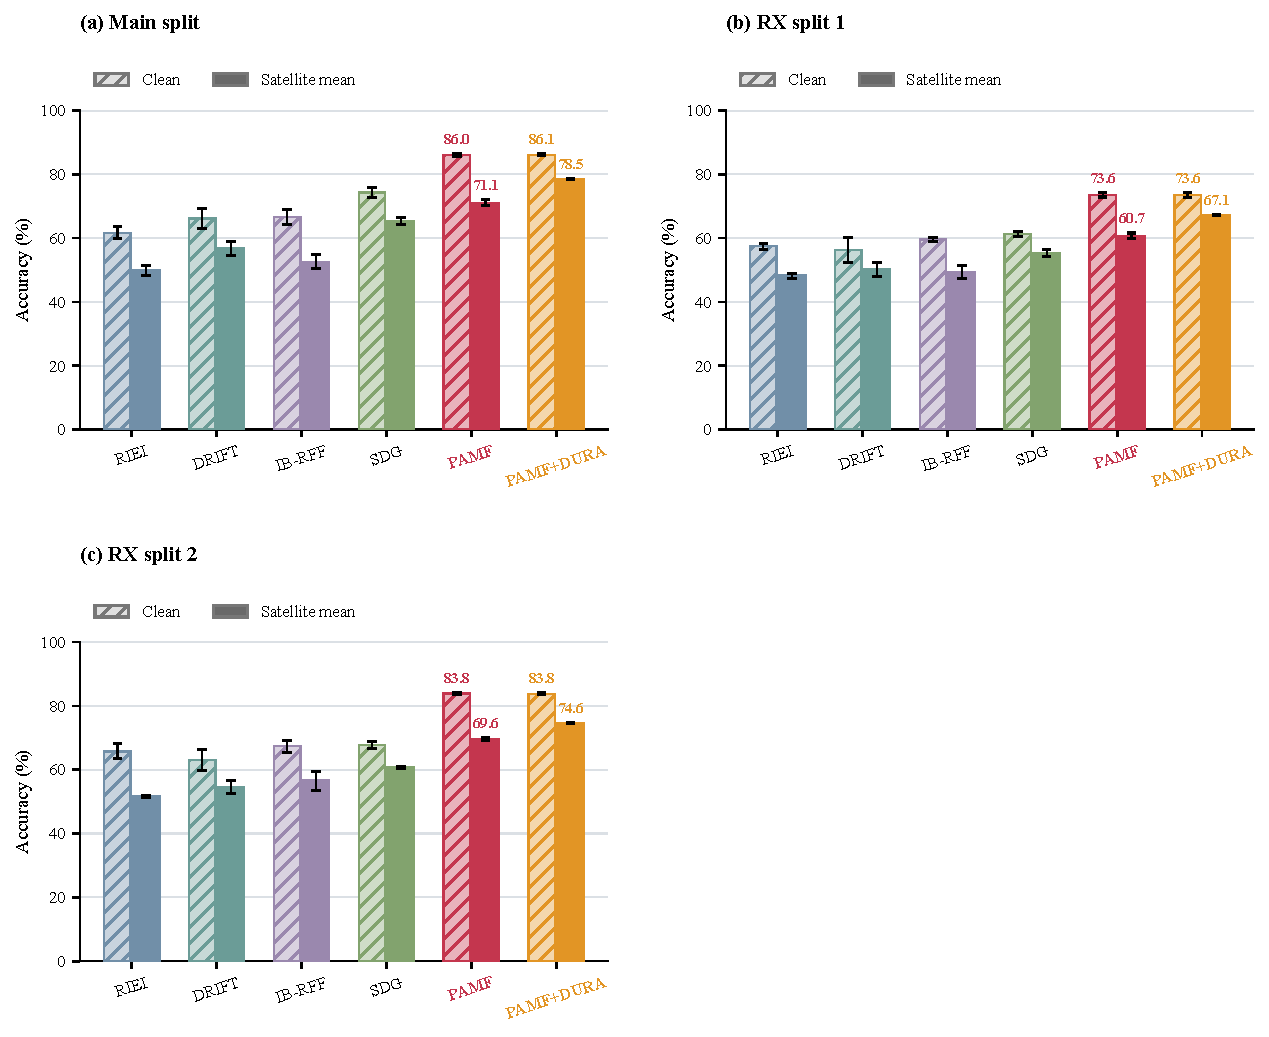
\includegraphics[width=\textwidth]{../figures/receiver_splits.pdf}
\caption{三套接收机划分的增强半监督结果：每种方法的左、右柱分别为 CLEAN 与综合星地。PAMF 和 PAMF+DURA 在全部面板保留。}
\label{fig:grouped-3}
\end{figure*}
\begin{figure*}[!tbp]
\centering
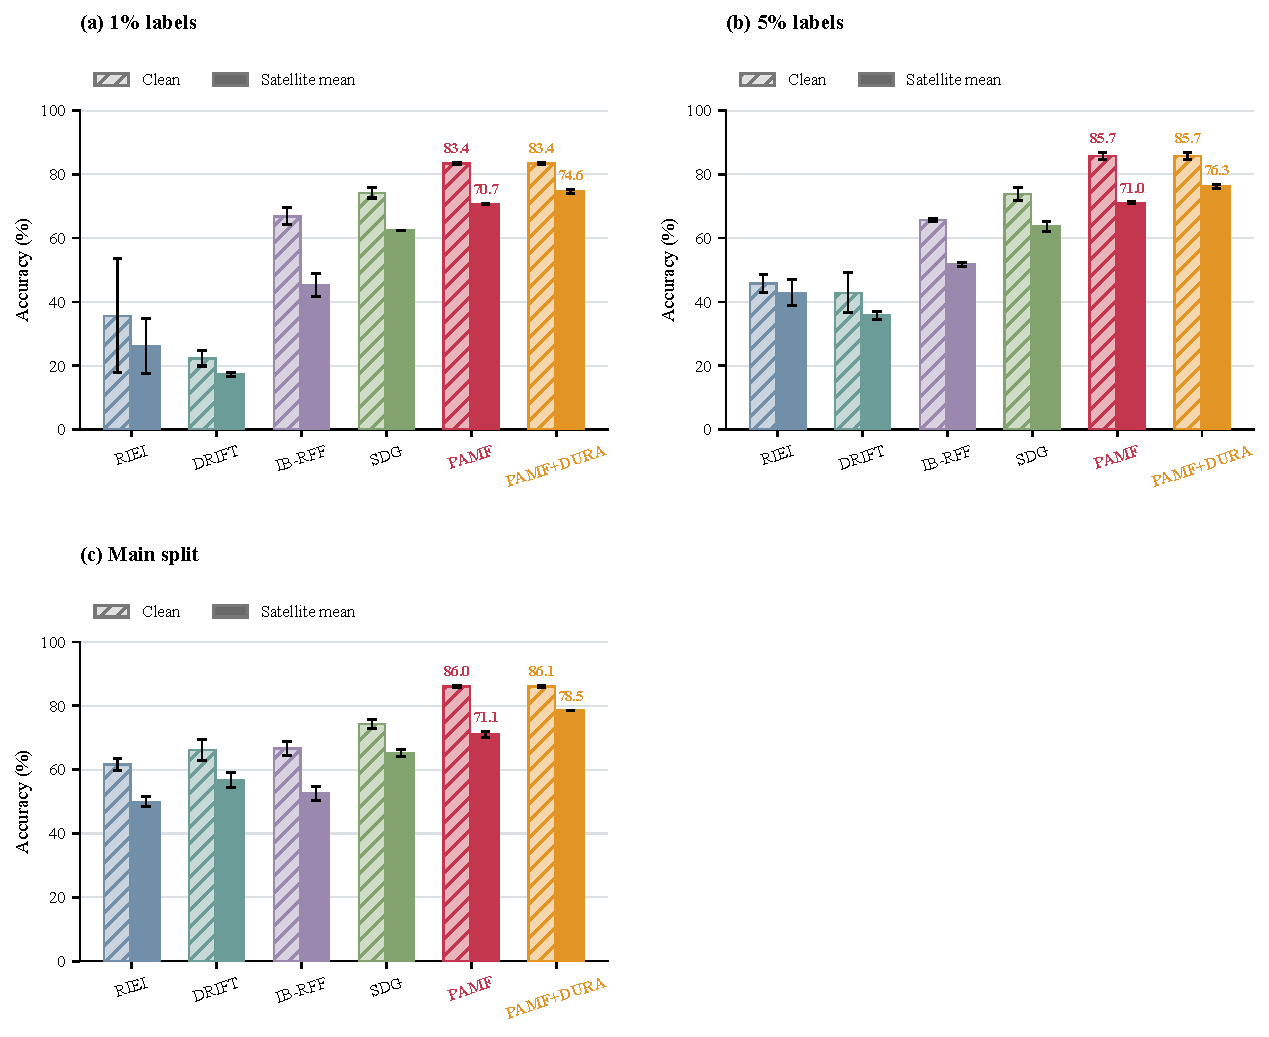
\includegraphics[width=\textwidth]{../figures/label_fraction.pdf}
\caption{1\%、5\%、10\% 标注比例的增强半监督结果，以 CLEAN／综合星地双柱比较六个主方法项。源验证量固定；保留非单调变化。}
\label{fig:grouped-4}
\end{figure*}
\begin{figure*}[!tbp]
\centering
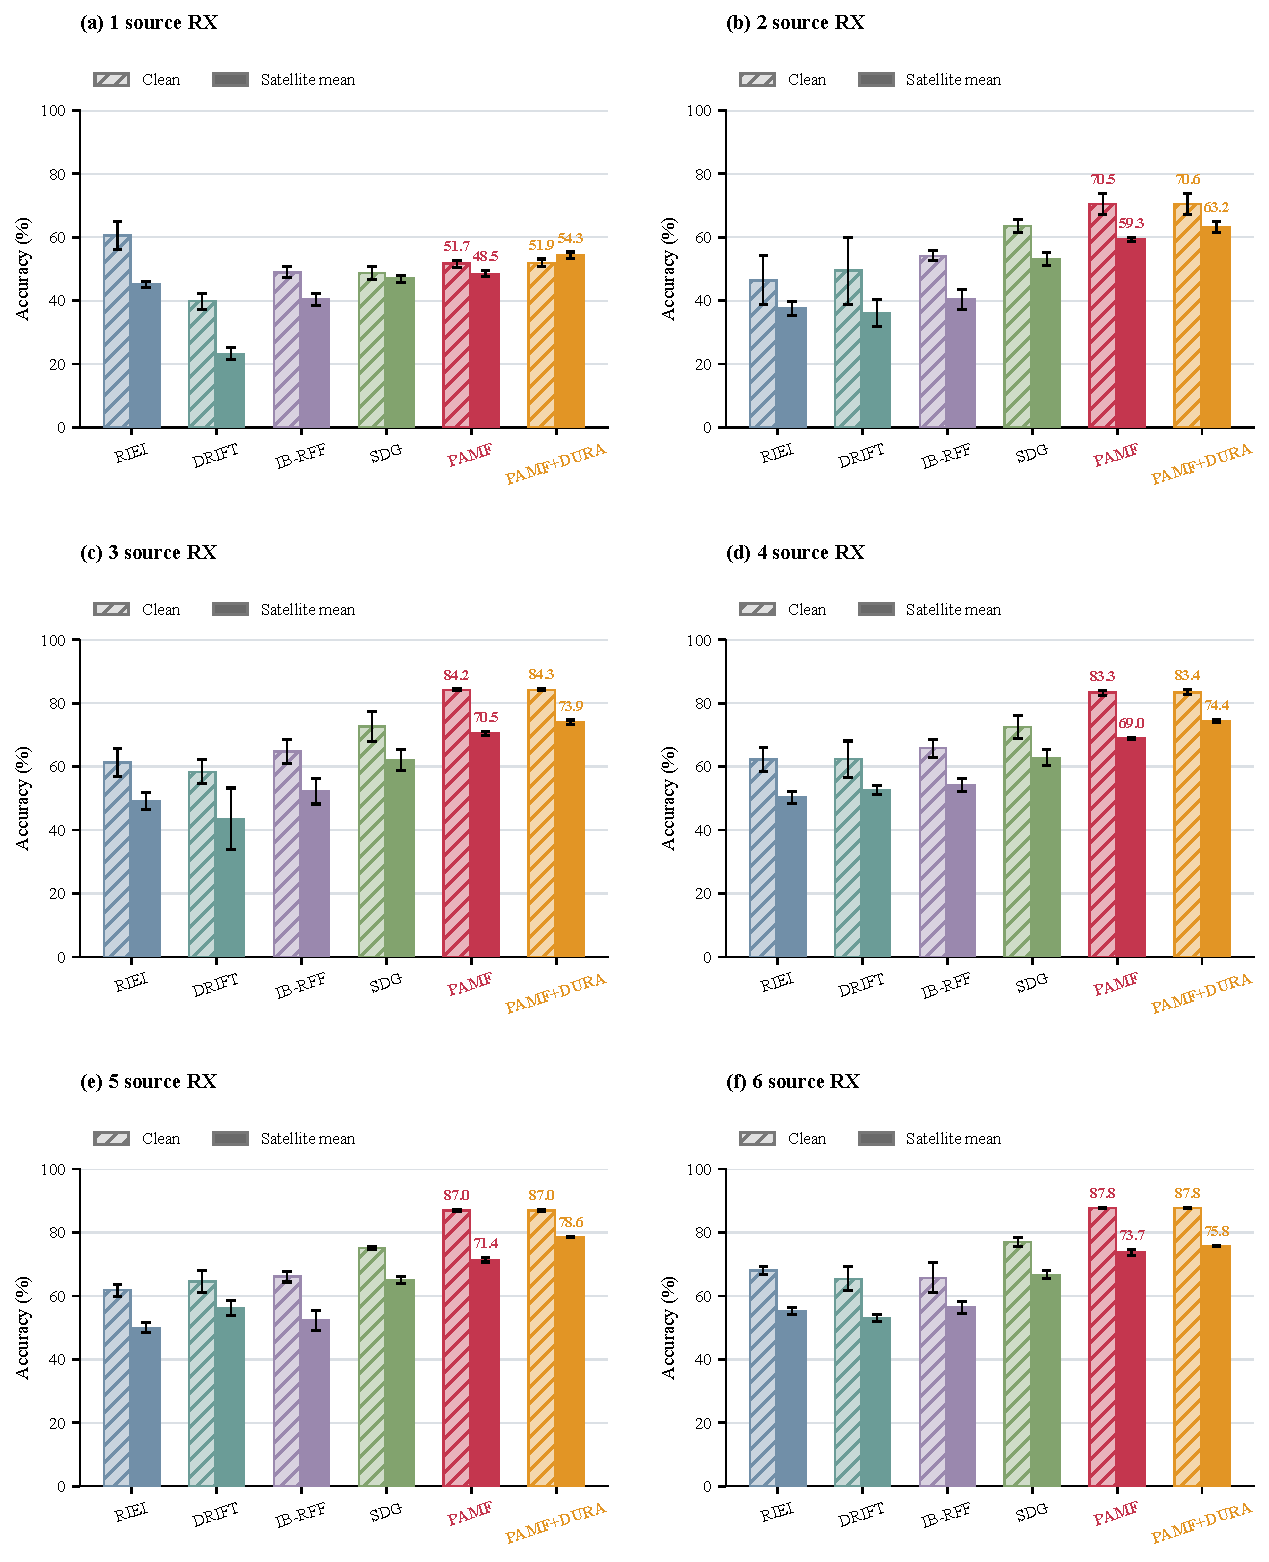
\includegraphics[width=\textwidth]{../figures/source_count_paired.pdf}
\caption{1 至 6 个源接收机的增强半监督双柱图，每种方法均给 CLEAN 和综合星地。全部面板使用共同 6 个目标接收机；5 源沿用同种子主实验模型，并由冻结逐接收机计数汇总。}
\label{fig:grouped-5}
\end{figure*}
\section{主实验的 CLEAN 与六种星地环境}
表~\ref{tab:grouped-5}~增强半监督主实验逐景准确率（\%）。

\begin{table*}[!tbp]
\caption{增强半监督主实验逐景准确率（\%）}
\label{tab:grouped-5}
\centering
\small
\begin{tabularx}{\textwidth}{YYYYYYY}
\toprule
\textbf{场景} & \textbf{RIEI} & \textbf{DRIFT} & \textbf{IB-RFF} & \textbf{SDG} & \textbf{PAMF} & \textbf{PAMF+DURA} \\
\midrule
CLEAN & 61.63\ensuremath{\pm}1.89 & 66.12\ensuremath{\pm}3.20 & 66.63\ensuremath{\pm}2.29 & 74.32\ensuremath{\pm}1.52 & 86.04\ensuremath{\pm}0.36 & 86.08\ensuremath{\pm}0.34 \\
高郊区 & 58.26\ensuremath{\pm}1.90 & 66.04\ensuremath{\pm}2.55 & 58.50\ensuremath{\pm}2.69 & 72.22\ensuremath{\pm}1.45 & 80.58\ensuremath{\pm}1.14 & 83.46\ensuremath{\pm}0.25 \\
中郊区 & 56.06\ensuremath{\pm}1.95 & 63.08\ensuremath{\pm}2.42 & 57.41\ensuremath{\pm}2.39 & 70.60\ensuremath{\pm}1.34 & 78.05\ensuremath{\pm}1.04 & 82.03\ensuremath{\pm}0.15 \\
低郊区 & 54.41\ensuremath{\pm}1.81 & 60.56\ensuremath{\pm}2.38 & 56.17\ensuremath{\pm}2.28 & 69.08\ensuremath{\pm}1.15 & 75.53\ensuremath{\pm}0.94 & 80.32\ensuremath{\pm}0.15 \\
高城市 & 54.85\ensuremath{\pm}1.78 & 62.62\ensuremath{\pm}2.55 & 56.12\ensuremath{\pm}2.53 & 69.64\ensuremath{\pm}1.33 & 77.18\ensuremath{\pm}1.07 & 82.19\ensuremath{\pm}0.18 \\
中城市 & 42.17\ensuremath{\pm}1.13 & 48.68\ensuremath{\pm}2.13 & 47.04\ensuremath{\pm}1.80 & 59.16\ensuremath{\pm}0.92 & 62.99\ensuremath{\pm}0.87 & 75.05\ensuremath{\pm}0.18 \\
低城市 & 33.96\ensuremath{\pm}0.74 & 39.55\ensuremath{\pm}1.80 & 40.17\ensuremath{\pm}1.40 & 51.11\ensuremath{\pm}0.69 & 51.98\ensuremath{\pm}0.46 & 68.05\ensuremath{\pm}0.25 \\
\bottomrule
\end{tabularx}
\end{table*}
\begin{figure*}[!tbp]
\centering
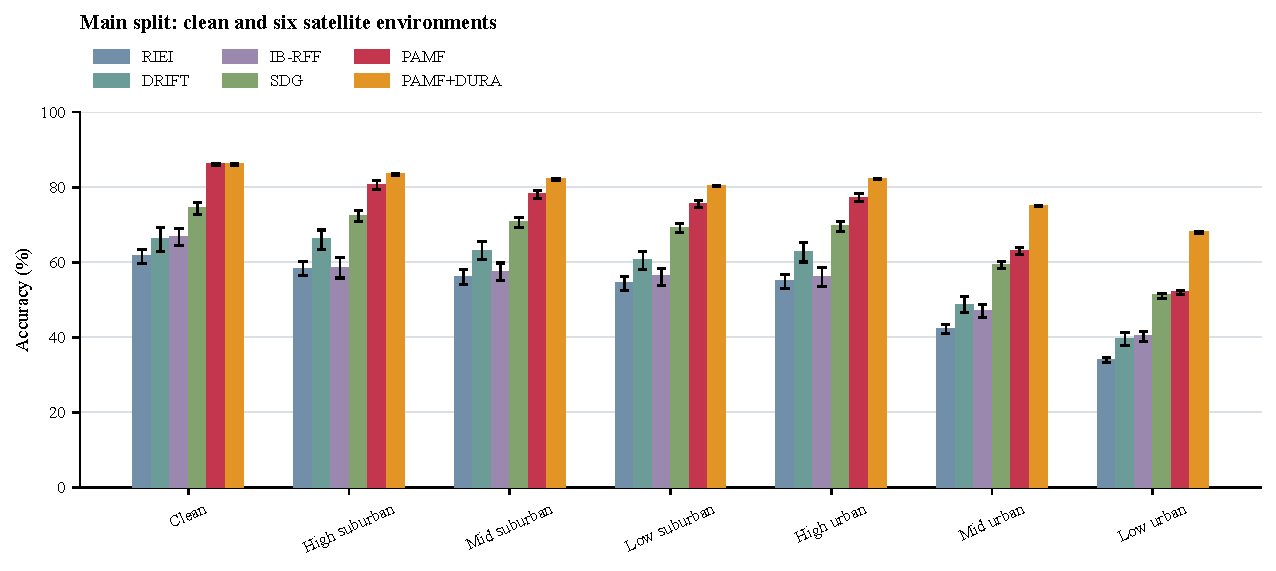
\includegraphics[width=\textwidth]{../figures/seven_scenes.pdf}
\caption{标准主划分、普通 PL 半监督＋增强的七场景结果。四种外部方法与单 PAMF 直接识别，PAMF+DURA 为恢复后识别；逐景单列 CLEAN 及六种 practical，不能以综合均值掩盖单景下降。}
\label{fig:grouped-6}
\end{figure*}
\section{1 至 6 个源接收机的折线}
5 个源接收机直接使用主对比实验的同种子模型，而不是另训模型。主实验原为 7 个目标接收机；其余源数量设置为共同 6 目标。为避免折线混入目标集合变化，本版从 5 源模型已经冻结的逐接收机统计中取共同 6 目标，按正确包数/总包数汇总：每个场景 108000 包。主表原 7 目标、每景 126000 包的成绩保持不变，也在 Excel 中保留。此操作仅重汇总冻结计数，没有重新预测或读取逐样本真值。

表~\ref{tab:grouped-6}~固定共同 6 目标的 CLEAN 准确率（\%）。

\begin{table*}[!tbp]
\caption{固定共同 6 目标的 CLEAN 准确率（\%）}
\label{tab:grouped-6}
\centering
\small
\begin{tabularx}{\textwidth}{YYYYYYY}
\toprule
\textbf{源接收机数} & \textbf{RIEI} & \textbf{DRIFT} & \textbf{IB-RFF} & \textbf{SDG} & \textbf{PAMF} & \textbf{PAMF+DURA} \\
\midrule
1 & 60.52\ensuremath{\pm}4.39 & 39.82\ensuremath{\pm}2.55 & 48.89\ensuremath{\pm}1.73 & 48.75\ensuremath{\pm}1.96 & 51.68\ensuremath{\pm}1.09 & 51.92\ensuremath{\pm}1.20 \\
2 & 46.39\ensuremath{\pm}7.74 & 49.47\ensuremath{\pm}10.58 & 54.10\ensuremath{\pm}1.59 & 63.62\ensuremath{\pm}1.99 & 70.49\ensuremath{\pm}3.30 & 70.56\ensuremath{\pm}3.30 \\
3 & 61.33\ensuremath{\pm}4.36 & 58.35\ensuremath{\pm}3.76 & 64.72\ensuremath{\pm}3.75 & 72.61\ensuremath{\pm}4.82 & 84.21\ensuremath{\pm}0.26 & 84.26\ensuremath{\pm}0.23 \\
4 & 62.27\ensuremath{\pm}3.71 & 62.39\ensuremath{\pm}5.68 & 65.79\ensuremath{\pm}2.81 & 72.48\ensuremath{\pm}3.61 & 83.32\ensuremath{\pm}0.83 & 83.40\ensuremath{\pm}0.79 \\
5 & 61.81\ensuremath{\pm}1.93 & 64.61\ensuremath{\pm}3.54 & 66.10\ensuremath{\pm}1.68 & 75.13\ensuremath{\pm}0.42 & 86.97\ensuremath{\pm}0.30 & 86.98\ensuremath{\pm}0.26 \\
6 & 68.05\ensuremath{\pm}1.20 & 65.43\ensuremath{\pm}3.75 & 65.76\ensuremath{\pm}4.70 & 77.05\ensuremath{\pm}1.37 & 87.81\ensuremath{\pm}0.10 & 87.84\ensuremath{\pm}0.10 \\
\bottomrule
\end{tabularx}
\end{table*}
\begin{figure*}[!tbp]
\centering
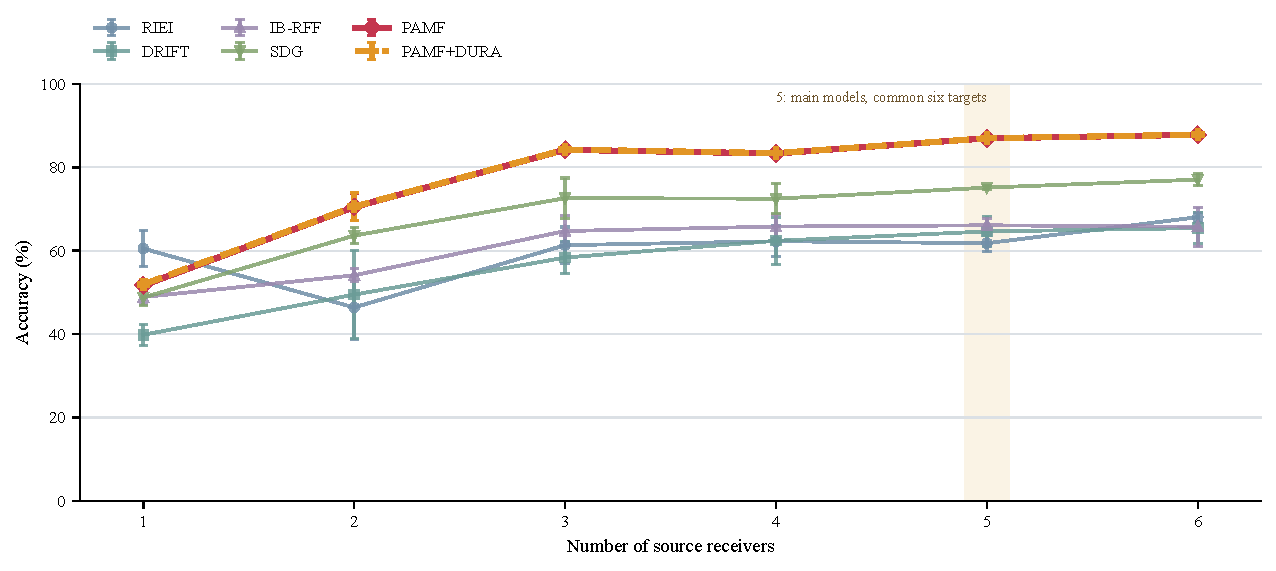
\includegraphics[width=\textwidth]{../figures/source_count_clean.pdf}
\caption{完整 1、2、3、4、5、6 源接收机折线：CLEAN。全部为增强半监督，固定共同 6 目标；5 源为同种子主实验模型的冻结计数重汇总。误差线为三种子样本标准差，保留非单调变化。}
\label{fig:grouped-7}
\end{figure*}
表~\ref{tab:grouped-7}~固定共同 6 目标的 综合星地 准确率（\%）。

\begin{table*}[!tbp]
\caption{固定共同 6 目标的 综合星地 准确率（\%）}
\label{tab:grouped-7}
\centering
\small
\begin{tabularx}{\textwidth}{YYYYYYY}
\toprule
\textbf{源接收机数} & \textbf{RIEI} & \textbf{DRIFT} & \textbf{IB-RFF} & \textbf{SDG} & \textbf{PAMF} & \textbf{PAMF+DURA} \\
\midrule
1 & 45.11\ensuremath{\pm}0.96 & 23.20\ensuremath{\pm}1.88 & 40.35\ensuremath{\pm}1.99 & 46.93\ensuremath{\pm}1.14 & 48.48\ensuremath{\pm}0.92 & 54.27\ensuremath{\pm}1.08 \\
2 & 37.56\ensuremath{\pm}2.13 & 36.05\ensuremath{\pm}4.27 & 40.44\ensuremath{\pm}3.12 & 53.11\ensuremath{\pm}2.01 & 59.25\ensuremath{\pm}0.64 & 63.19\ensuremath{\pm}1.69 \\
3 & 49.20\ensuremath{\pm}2.74 & 43.50\ensuremath{\pm}9.74 & 52.22\ensuremath{\pm}4.01 & 62.09\ensuremath{\pm}3.38 & 70.50\ensuremath{\pm}0.66 & 73.94\ensuremath{\pm}0.76 \\
4 & 50.23\ensuremath{\pm}1.96 & 52.59\ensuremath{\pm}1.52 & 54.22\ensuremath{\pm}2.12 & 62.75\ensuremath{\pm}2.54 & 68.97\ensuremath{\pm}0.32 & 74.39\ensuremath{\pm}0.59 \\
5 & 49.99\ensuremath{\pm}1.55 & 56.14\ensuremath{\pm}2.33 & 52.22\ensuremath{\pm}3.20 & 65.07\ensuremath{\pm}1.06 & 71.43\ensuremath{\pm}0.72 & 78.63\ensuremath{\pm}0.24 \\
6 & 55.25\ensuremath{\pm}1.07 & 52.96\ensuremath{\pm}1.06 & 56.40\ensuremath{\pm}1.87 & 66.69\ensuremath{\pm}1.28 & 73.69\ensuremath{\pm}0.88 & 75.77\ensuremath{\pm}0.13 \\
\bottomrule
\end{tabularx}
\end{table*}
\begin{figure*}[!tbp]
\centering
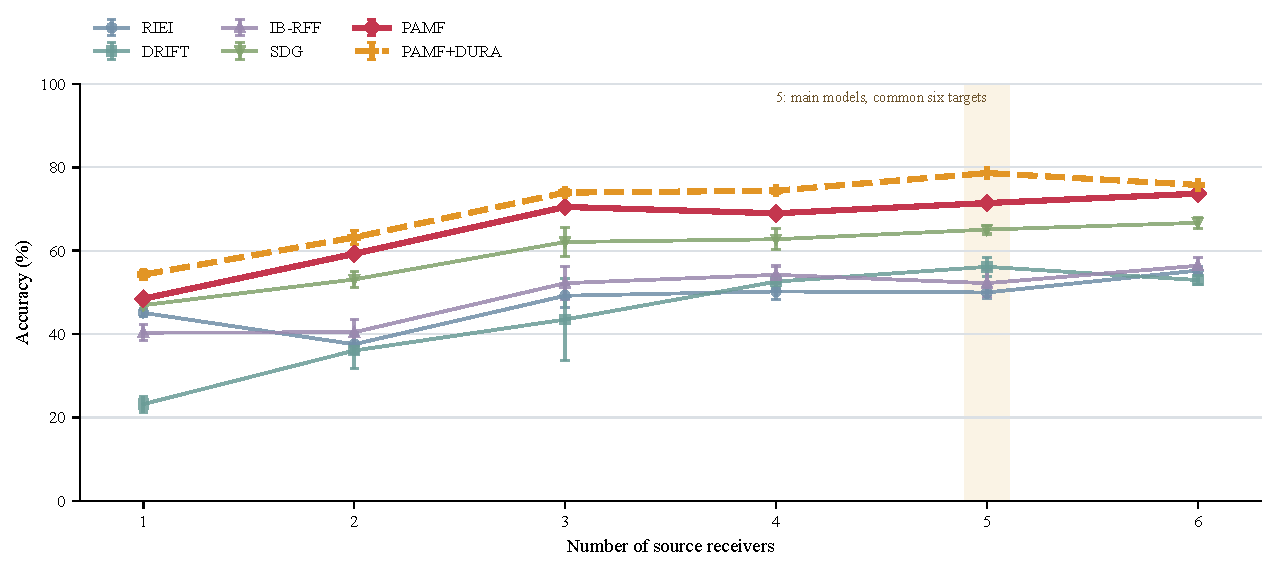
\includegraphics[width=\textwidth]{../figures/source_count_practical.pdf}
\caption{完整 1、2、3、4、5、6 源接收机折线：综合星地。全部为增强半监督，固定共同 6 目标；5 源为同种子主实验模型的冻结计数重汇总。误差线为三种子样本标准差，保留非单调变化。}
\label{fig:grouped-8}
\end{figure*}
源训练量随源接收机数量自然增长，因此折线同时反映接收机覆盖与训练记录量变化，不是固定样本预算下仅接收机多样性的因果效应。各设置仍使用原冻结测试的场景配置。

\section{包含 PAMF 的 DURA 泛用性}
表~\ref{tab:grouped-8}~标准主划分、增强半监督、综合星地的恢复前后配对。

\begin{table*}[!tbp]
\caption{标准主划分、增强半监督、综合星地的恢复前后配对}
\label{tab:grouped-8}
\centering
\small
\begin{tabularx}{\textwidth}{YYYY}
\toprule
\textbf{识别方法} & \textbf{未接 DURA（\%）} & \textbf{接入 DURA（\%）} & \textbf{配对变化（百分点）} \\
\midrule
RIEI & 49.95 & 56.73 & +6.77\ensuremath{\pm}0.89 \\
DRIFT & 56.76 & 60.75 & +4.00\ensuremath{\pm}4.28 \\
IB-RFF & 52.57 & 62.21 & +9.64\ensuremath{\pm}1.42 \\
SDG & 65.30 & 67.12 & +1.82\ensuremath{\pm}1.87 \\
PAMF & 71.05 & 78.52 & +7.47\ensuremath{\pm}0.79 \\
\bottomrule
\end{tabularx}
\end{table*}
\begin{figure*}[!tbp]
\centering
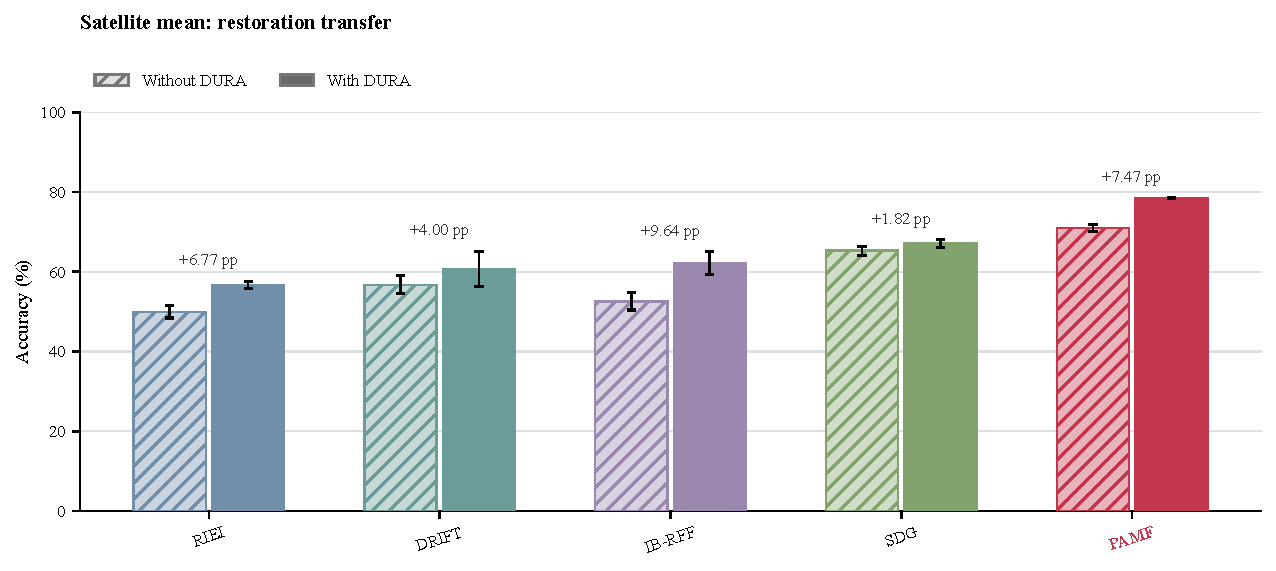
\includegraphics[width=\textwidth]{../figures/DURA_generality.pdf}
\caption{DURA 泛用性采用双柱，五种识别器均包括在内：RIEI、DRIFT、IB-RFF、SDG、PAMF。每种方法固定同一识别器、样本、场景和种子，只切换是否先恢复；柱顶标种子内配对百分点变化。全部为增强半监督、标准主划分的综合星地测试。}
\label{fig:grouped-9}
\end{figure*}
所有恢复后结果都使用匹配同一数据契约的恢复器。三个识别器种子共享一份匹配恢复器，不能称为三套独立完整系统。泛用性收益是识别器接入固定恢复网络的测试收益，不证明恢复器对每个方法、每个场景都提高。

\section{保留资料与明确缺项}
Excel 前 9 个工作表对应本报告重点图，共 19 个面板；后 26 个补充工作表保留此前的监督分组、半监督分组、十类规模、Macro-F1、双跨/跨日诊断、完整逐景、时延、覆盖与逐模型登记，并补入原两套 11 设置 DURA 面板。工作簿共 35 个工作表、51 个可编辑图表。每个重点实验页都有目的、设置、对应数据划分、图表数据、三种子数值和完整结果。

当前普通 PL 配方的无增强 PAMF 仍是缺项，已获用户确认先交付已有证据。没有启动新增训练、预测、真值评分或 DURA 训练。当前方法自身消融的其他缺项仍按原报告记录，不把旧复杂半监督或已退出方法改名为普通 PL。旧报告与不可覆盖导出包均保留。

\FloatBarrier
\appendices
\section{阅读名称与原始记录的对应}
当前主方法来自既有 practical residual 完整对比包及 PAMF 监督/ordinary\_PL 完成矩阵。新增补入的无增强监督 PAMF 来自 \nolinkurl{20261024-practical-residual-full2x2-complete-r14.zip} 的 PAMF 监督 A 组；其当前普通 PL 对照未完成。5 源曲线使用同种子 F0 主模型，仅从冻结的接收机统计中选择预先指定的共同目标集合 [0,2,5,7,9,10] 汇总。没有根据目标成绩筛接收机或挑模型。

导出包包含逐图来源表、冻结种子统计、共同 6 目标正确/总包计数、IEEE 源码、PDF/SVG/PNG 和纯标准库复核器。先按种子汇总六景和配对差，再计算跨种子样本标准差；缺失结果保持缺失。正文采用识别器、恢复器和数据设置的可读名称，原始编号只在机器可读追溯数据中保留。

\FloatBarrier
\end{document}
